% Editable source for result.pdf, written by make_figures.py from
% run_github_38776966036/panel/result.json. Ratios with 95% paired bootstrap intervals
% (frozen protocol.json statistics); log2 axis; dashed line = parity.
\documentclass[tikz,border=6pt]{standalone}
\usepackage[T1]{fontenc}
\begin{document}
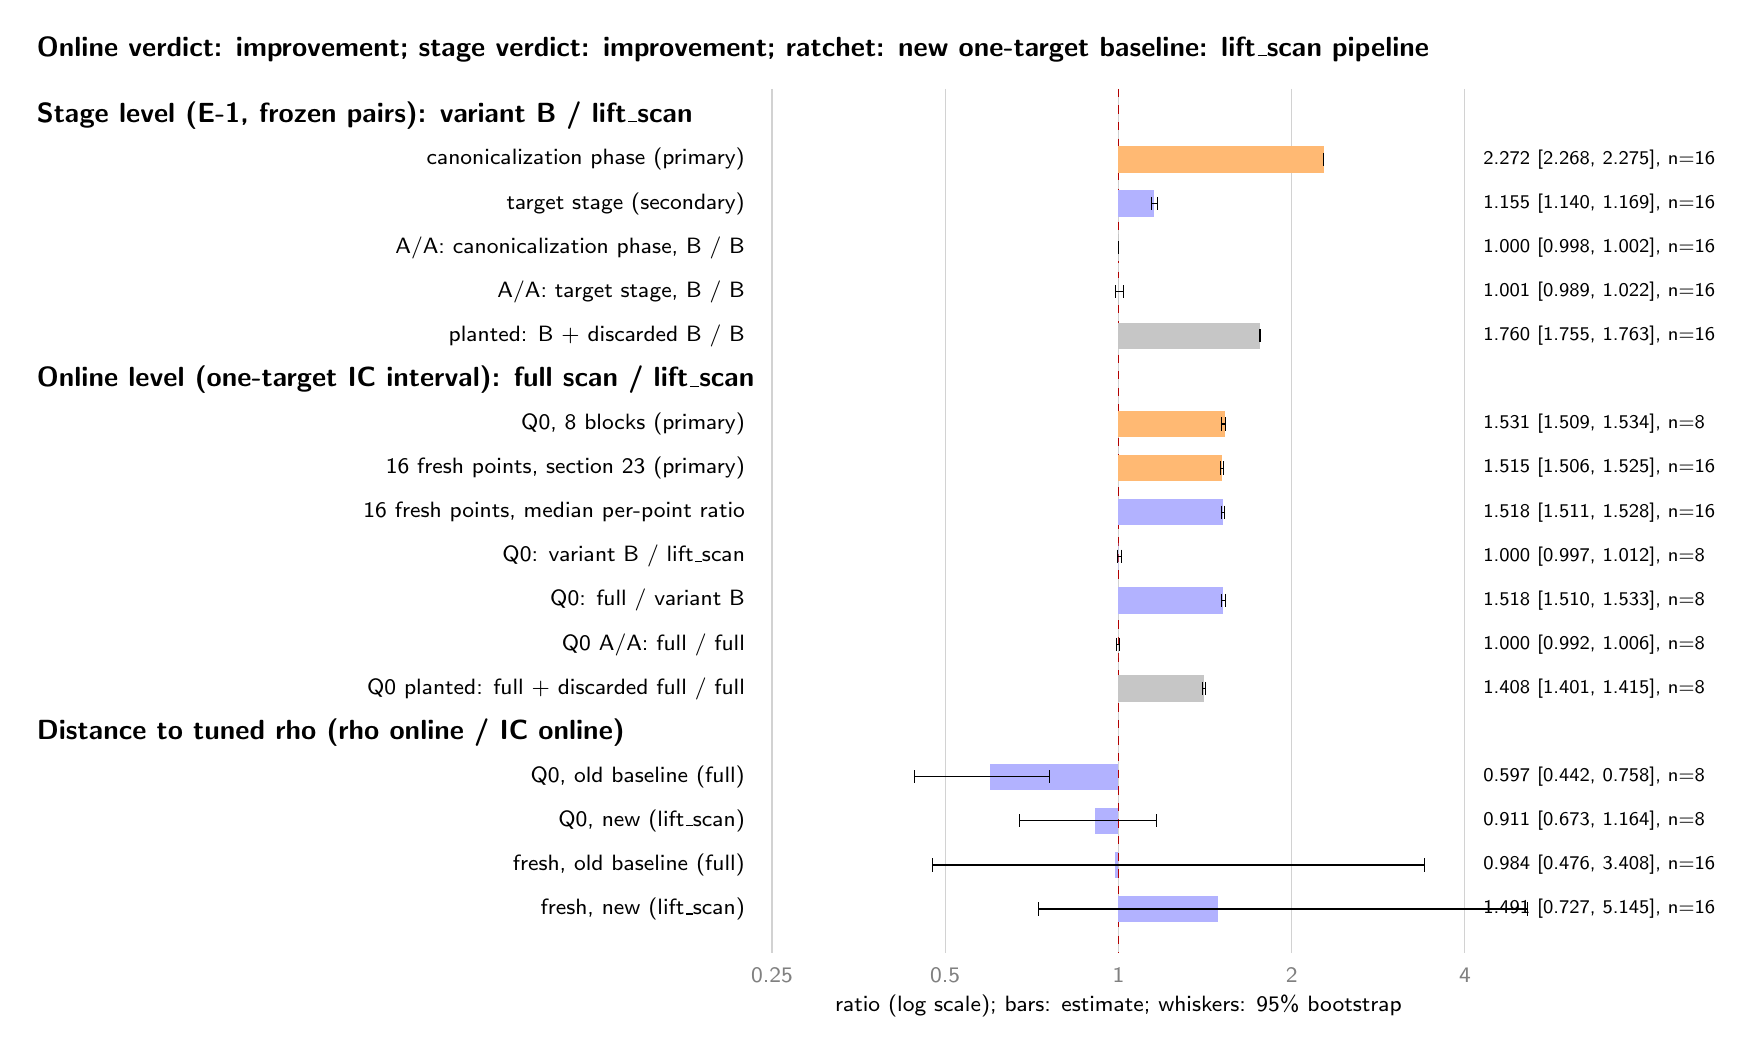
\begin{tikzpicture}[font=\sffamily\footnotesize,x=22mm,y=-5.6mm]
\draw[gray!35] (-2.0000,-0.6) -- (-2.0000,19); \node[gray] at (-2.0000,19.5) {0.25};
\draw[gray!35] (-1.0000,-0.6) -- (-1.0000,19); \node[gray] at (-1.0000,19.5) {0.5};
\draw[gray!35] (0.0000,-0.6) -- (0.0000,19); \node[gray] at (0.0000,19.5) {1};
\draw[gray!35] (1.0000,-0.6) -- (1.0000,19); \node[gray] at (1.0000,19.5) {2};
\draw[gray!35] (2.0000,-0.6) -- (2.0000,19); \node[gray] at (2.0000,19.5) {4};
\draw[red!70!black,dashed] (0,-0.6) -- (0,19);
\node at (0,20.2) {ratio (log scale); bars: estimate; whiskers: 95\% bootstrap};
\node[anchor=west,font=\sffamily\bfseries] at (-6.3,-1.5) {Online verdict: improvement; stage verdict: improvement; ratchet: new one-target baseline: lift\_scan pipeline};
\node[anchor=west,font=\sffamily\bfseries] at (-6.3,0) {Stage level (E-1, frozen pairs): variant B / lift\_scan};
\node[anchor=east] at (-2.1000,1) {canonicalization phase (primary)};
\fill[orange!55] (0,0.700000) rectangle (1.1842,1.300000);
\draw (1.1816,1) -- (1.1857,1); \draw (1.1816,0.850000) -- (1.1816,1.150000); \draw (1.1857,0.850000) -- (1.1857,1.150000);
\node[anchor=west,font=\sffamily\scriptsize] at (2.0500,1) {2.272 [2.268, 2.275], n=16};
\node[anchor=east] at (-2.1000,2) {target stage (secondary)};
\fill[blue!30] (0,1.700000) rectangle (0.2078,2.300000);
\draw (0.1896,2) -- (0.2247,2); \draw (0.1896,1.850000) -- (0.1896,2.150000); \draw (0.2247,1.850000) -- (0.2247,2.150000);
\node[anchor=west,font=\sffamily\scriptsize] at (2.0500,2) {1.155 [1.140, 1.169], n=16};
\node[anchor=east] at (-2.1000,3) {A/A: canonicalization phase, B / B};
\fill[gray!45] (0,2.700000) rectangle (0.0003,3.300000);
\draw (-0.0022,3) -- (0.0023,3); \draw (-0.0022,2.850000) -- (-0.0022,3.150000); \draw (0.0023,2.850000) -- (0.0023,3.150000);
\node[anchor=west,font=\sffamily\scriptsize] at (2.0500,3) {1.000 [0.998, 1.002], n=16};
\node[anchor=east] at (-2.1000,4) {A/A: target stage, B / B};
\fill[gray!45] (0,3.700000) rectangle (0.0015,4.300000);
\draw (-0.0156,4) -- (0.0315,4); \draw (-0.0156,3.850000) -- (-0.0156,4.150000); \draw (0.0315,3.850000) -- (0.0315,4.150000);
\node[anchor=west,font=\sffamily\scriptsize] at (2.0500,4) {1.001 [0.989, 1.022], n=16};
\node[anchor=east] at (-2.1000,5) {planted: B + discarded B / B};
\fill[gray!45] (0,4.700000) rectangle (0.8152,5.300000);
\draw (0.8117,5) -- (0.8179,5); \draw (0.8117,4.850000) -- (0.8117,5.150000); \draw (0.8179,4.850000) -- (0.8179,5.150000);
\node[anchor=west,font=\sffamily\scriptsize] at (2.0500,5) {1.760 [1.755, 1.763], n=16};
\node[anchor=west,font=\sffamily\bfseries] at (-6.3,6) {Online level (one-target IC interval): full scan / lift\_scan};
\node[anchor=east] at (-2.1000,7) {Q0, 8 blocks (primary)};
\fill[orange!55] (0,6.700000) rectangle (0.6144,7.300000);
\draw (0.5939,7) -- (0.6169,7); \draw (0.5939,6.850000) -- (0.5939,7.150000); \draw (0.6169,6.850000) -- (0.6169,7.150000);
\node[anchor=west,font=\sffamily\scriptsize] at (2.0500,7) {1.531 [1.509, 1.534], n=8};
\node[anchor=east] at (-2.1000,8) {16 fresh points, section 23 (primary)};
\fill[orange!55] (0,7.700000) rectangle (0.5995,8.300000);
\draw (0.5908,8) -- (0.6085,8); \draw (0.5908,7.850000) -- (0.5908,8.150000); \draw (0.6085,7.850000) -- (0.6085,8.150000);
\node[anchor=west,font=\sffamily\scriptsize] at (2.0500,8) {1.515 [1.506, 1.525], n=16};
\node[anchor=east] at (-2.1000,9) {16 fresh points, median per-point ratio};
\fill[blue!30] (0,8.700000) rectangle (0.6021,9.300000);
\draw (0.5950,9) -- (0.6115,9); \draw (0.5950,8.850000) -- (0.5950,9.150000); \draw (0.6115,8.850000) -- (0.6115,9.150000);
\node[anchor=west,font=\sffamily\scriptsize] at (2.0500,9) {1.518 [1.511, 1.528], n=16};
\node[anchor=east] at (-2.1000,10) {Q0: variant B / lift\_scan};
\fill[blue!30] (0,9.700000) rectangle (-0.0001,10.300000);
\draw (-0.0049,10) -- (0.0169,10); \draw (-0.0049,9.850000) -- (-0.0049,10.150000); \draw (0.0169,9.850000) -- (0.0169,10.150000);
\node[anchor=west,font=\sffamily\scriptsize] at (2.0500,10) {1.000 [0.997, 1.012], n=8};
\node[anchor=east] at (-2.1000,11) {Q0: full / variant B};
\fill[blue!30] (0,10.700000) rectangle (0.6024,11.300000);
\draw (0.5944,11) -- (0.6160,11); \draw (0.5944,10.850000) -- (0.5944,11.150000); \draw (0.6160,10.850000) -- (0.6160,11.150000);
\node[anchor=west,font=\sffamily\scriptsize] at (2.0500,11) {1.518 [1.510, 1.533], n=8};
\node[anchor=east] at (-2.1000,12) {Q0 A/A: full / full};
\fill[gray!45] (0,11.700000) rectangle (-0.0000,12.300000);
\draw (-0.0115,12) -- (0.0083,12); \draw (-0.0115,11.850000) -- (-0.0115,12.150000); \draw (0.0083,11.850000) -- (0.0083,12.150000);
\node[anchor=west,font=\sffamily\scriptsize] at (2.0500,12) {1.000 [0.992, 1.006], n=8};
\node[anchor=east] at (-2.1000,13) {Q0 planted: full + discarded full / full};
\fill[gray!45] (0,12.700000) rectangle (0.4937,13.300000);
\draw (0.4869,13) -- (0.5004,13); \draw (0.4869,12.850000) -- (0.4869,13.150000); \draw (0.5004,12.850000) -- (0.5004,13.150000);
\node[anchor=west,font=\sffamily\scriptsize] at (2.0500,13) {1.408 [1.401, 1.415], n=8};
\node[anchor=west,font=\sffamily\bfseries] at (-6.3,14) {Distance to tuned rho (rho online / IC online)};
\node[anchor=east] at (-2.1000,15) {Q0, old baseline (full)};
\fill[blue!30] (0,14.700000) rectangle (-0.7442,15.300000);
\draw (-1.1773,15) -- (-0.3993,15); \draw (-1.1773,14.850000) -- (-1.1773,15.150000); \draw (-0.3993,14.850000) -- (-0.3993,15.150000);
\node[anchor=west,font=\sffamily\scriptsize] at (2.0500,15) {0.597 [0.442, 0.758], n=8};
\node[anchor=east] at (-2.1000,16) {Q0, new (lift\_scan)};
\fill[blue!30] (0,15.700000) rectangle (-0.1348,16.300000);
\draw (-0.5703,16) -- (0.2192,16); \draw (-0.5703,15.850000) -- (-0.5703,16.150000); \draw (0.2192,15.850000) -- (0.2192,16.150000);
\node[anchor=west,font=\sffamily\scriptsize] at (2.0500,16) {0.911 [0.673, 1.164], n=8};
\node[anchor=east] at (-2.1000,17) {fresh, old baseline (full)};
\fill[blue!30] (0,16.700000) rectangle (-0.0228,17.300000);
\draw (-1.0711,17) -- (1.7691,17); \draw (-1.0711,16.850000) -- (-1.0711,17.150000); \draw (1.7691,16.850000) -- (1.7691,17.150000);
\node[anchor=west,font=\sffamily\scriptsize] at (2.0500,17) {0.984 [0.476, 3.408], n=16};
\node[anchor=east] at (-2.1000,18) {fresh, new (lift\_scan)};
\fill[blue!30] (0,17.700000) rectangle (0.5767,18.300000);
\draw (-0.4600,18) -- (2.3630,18); \draw (-0.4600,17.850000) -- (-0.4600,18.150000); \draw (2.3630,17.850000) -- (2.3630,18.150000);
\node[anchor=west,font=\sffamily\scriptsize] at (2.0500,18) {1.491 [0.727, 5.145], n=16};
\end{tikzpicture}
\end{document}
